% Chapter 9. Task states, and which ones you can leave.
\documentclass[tikz,border=6pt]{standalone}
% Shared look for every TikZ figure in the book.
% Colours match book/preamble.tex exactly. Change both or neither.

\usepackage{tikz}
\usepackage{xcolor}
\usepackage{amsmath}
\IfFileExists{libertinus.sty}{\usepackage[mono=false]{libertinus}}{}
\IfFileExists{inconsolata.sty}{\usepackage[varqu,varl,scaled=0.95]{inconsolata}}{}

\usetikzlibrary{
  arrows.meta, positioning, calc, fit, backgrounds, shapes.geometric,
  shapes.misc, decorations.pathreplacing, decorations.pathmorphing,
  patterns, chains, matrix, shadows.blur
}

\definecolor{ink}{HTML}{15181D}
\definecolor{muted}{HTML}{5B6472}
\definecolor{rule}{HTML}{C9CED6}
\definecolor{wash}{HTML}{F4F5F7}
\definecolor{accent}{HTML}{0F5C8C}
\definecolor{accentsoft}{HTML}{E7F0F6}
\definecolor{warm}{HTML}{B4531A}
\definecolor{warmsoft}{HTML}{FBF0E7}
\definecolor{good}{HTML}{2C6E49}
\definecolor{goodsoft}{HTML}{E9F2EC}
\definecolor{danger}{HTML}{9B2226}
\definecolor{dangersoft}{HTML}{FAECEC}

\tikzset{
  font=\sffamily\small,
  >={Stealth[length=5pt, width=4pt]},
  %
  box/.style={
    draw=rule, line width=0.8pt, fill=wash, rounded corners=2pt,
    inner sep=7pt, align=center, text=ink, minimum height=9mm,
  },
  boxa/.style={box, draw=accent, fill=accentsoft},
  boxg/.style={box, draw=good,   fill=goodsoft},
  boxw/.style={box, draw=warm,   fill=warmsoft},
  boxd/.style={box, draw=danger, fill=dangersoft},
  %
  lane/.style={draw=rule, line width=0.7pt, fill=white, rounded corners=2pt,
               inner sep=6pt, align=center, minimum width=26mm},
  %
  flow/.style={draw=accent, line width=1.0pt, ->},
  flowback/.style={flow, densely dashed},
  flowmuted/.style={draw=muted, line width=0.8pt, ->},
  lifeline/.style={draw=rule, line width=0.7pt, densely dotted},
  %
  lbl/.style={font=\sffamily\scriptsize, text=muted, inner sep=2pt},
  lblink/.style={font=\sffamily\scriptsize, text=ink, inner sep=2pt},
  tag/.style={font=\ttfamily\scriptsize, text=accent, inner sep=2pt,
              fill=white, inner xsep=3pt},
  note/.style={font=\sffamily\scriptsize\itshape, text=muted, align=left},
  %
  band/.style={draw=none, rounded corners=1pt},
  tick/.style={draw=muted, line width=0.6pt},
}

% A horizontal timeline bar segment: \barseg{x0}{x1}{y}{colour}{label}
\newcommand{\barseg}[5]{%
  \fill[#4, rounded corners=1pt] (#1,#3-0.16) rectangle (#2,#3+0.16);
  \node[lbl, text=white, font=\sffamily\scriptsize\bfseries]
       at ({(#1+#2)/2},#3) {#5};
}

\begin{document}
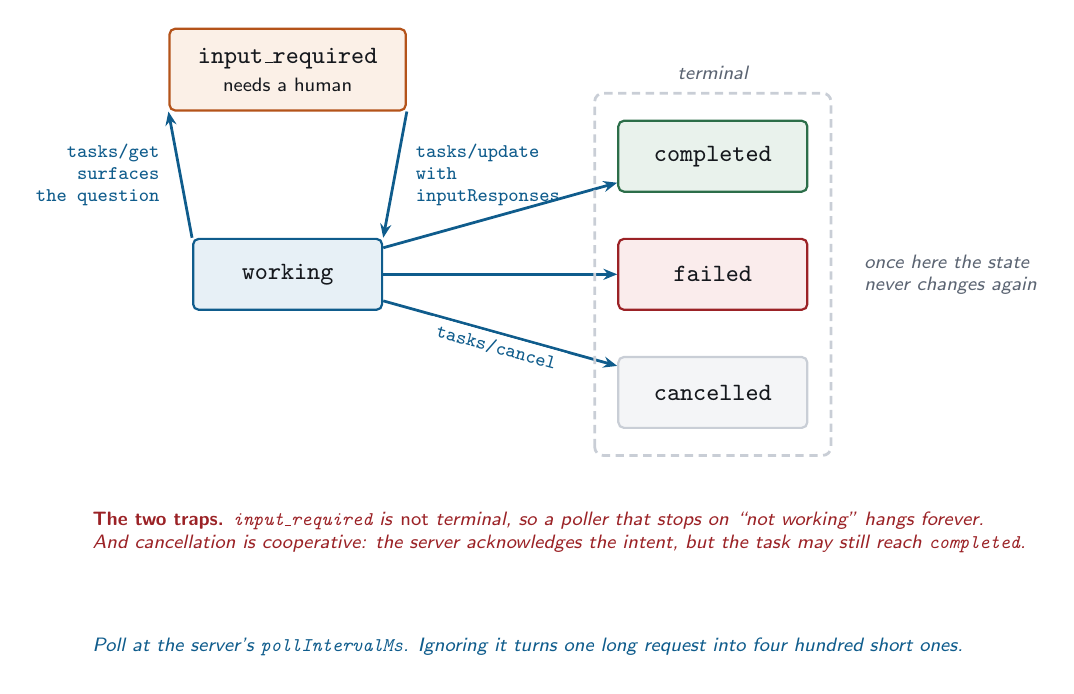
\begin{tikzpicture}[x=1cm, y=1cm, node distance=1cm]

  \node[boxa, minimum width=24mm] (working) at (0,0) {\texttt{working}};
  \node[boxw, minimum width=30mm, align=center] (input) at (0,2.6)
    {\texttt{input\_required}\\[-1pt]\scriptsize needs a human};

  \node[boxg, minimum width=24mm] (done)   at (5.4,1.5) {\texttt{completed}};
  \node[boxd, minimum width=24mm] (failed) at (5.4,0.0) {\texttt{failed}};
  \node[box,  minimum width=24mm] (cancel) at (5.4,-1.5) {\texttt{cancelled}};

  % Two arrows between the same pair of nodes, kept apart by anchoring to
  % opposite corners so their labels cannot collide.
  \draw[flow] (working.north west) -- (input.south west)
    node[tag, midway, left, align=right, xshift=-4pt]
    {\texttt{tasks/get}\\surfaces\\the question};
  \draw[flow] (input.south east) -- (working.north east)
    node[tag, midway, right, align=left, xshift=4pt]
    {\texttt{tasks/update}\\with\\inputResponses};

  \draw[flow] (working) -- (done);
  \draw[flow] (working) -- (failed);
  \draw[flow] (working) -- node[tag, below, sloped] {tasks/cancel} (cancel);

  % terminal bracket
  \draw[draw=rule, line width=1pt, densely dashed, rounded corners=3pt]
    (3.9,-2.3) rectangle (6.9,2.3);
  \node[note, anchor=south, text=muted] at (5.4,2.35) {terminal};

  \node[note, anchor=west, align=left, text=muted] at (7.2,0.0)
    {once here the state\\never changes again};

  \node[note, anchor=north west, align=left, text=danger] at (-2.6,-2.9)
    {\textbf{The two traps.}
     \texttt{input\_required} is \emph{not} terminal, so a poller that stops on
     ``not working'' hangs forever.\\
     And cancellation is cooperative: the server acknowledges the intent, but
     the task may still reach \texttt{completed}.};

  \node[note, anchor=north west, align=left, text=accent] at (-2.6,-4.5)
    {Poll at the server's \texttt{pollIntervalMs}. Ignoring it turns one long
     request into four hundred short ones.};

\end{tikzpicture}
\end{document}
